% Szglab4
% ===========================================================================
%
\chapter{Analízis modell kidolgozása 2}

\thispagestyle{fancy}

\section{Objektum katalógus}

\subsection{Glue}
A „Glue” objektum megvalósít egy adott tulajdonságú akadályt. Amely robot belemegy, annak a sebességét megfelezi. 
\subsection{GUI}
A grafikus felületet megvalósító objektum. Ez az objektum maga a menü, ami a játék indítása után ugrik fel. Itt találhatóak a beállítások (mint például a gondolkodás idő és a maximális játék idő vagy a körök száma) és a játékmódok. Gombnyomásra fogja elindítani a játék működési szálát. Ez az objektum kezeli az ablak eseményeit és a játék bezárását.
\subsection{HUD}
Ez az objektum követi és nyilvántartja, hogy a robotok hány checkpoint-on mentek át, mennyi olaj és ragacs van náluk amit felhasználhatnak, illetve kiírja a képernyőre a hátramaradó időt és a megtett körök számát. Feladata, hogy minden körben megvizsgálja, hogy a robotok elérték-e a következő checkpointot.
\subsection{MapBuilder}
Fájlból beolvassa és létrehozza a memóriában a pályát, a kezdő pozíciókat és a checkpointokat reprezentáló objektumokat.  Mivel a  MapBuilder objektum tárolja a pályát így feladat, hogy vizsgálja a robotok azon belül tartózkodását.  
\subsection{Oil}
Ez az objektum az Obstacle osztály leszármazottja. Hasonlóan a Glue objektumhoz, egy adott hatást valósít meg, ami letiltja a következő körben történő irányítását a robotnak, ami belelépett.
\subsection{Phoebe}
A játék logikát megvalósító objektum. Listában tárolja a pályán tartózkodó robotokat, akadályokat és figyeli, hogy mikor ér véget a játék. A „Phoebe” objektum rajzolja ki az objektumokat a pályán és szálként indítható osztályt, melyben maga a játék fut. Játékindításkor berakja a pályára a robotokat és az akadályokat a kezdő pozíciókba. Ebben az objektumban történnek az ellenőrzések (akadályba vagy robotba ütközések, pályáról leesés).
\subsection{Robot}
Olyan objektum, mely a pályán található robotokat valósítja meg. Leírja a viselkedésüket és a kezelésüket. A „Robot” osztály a Unit-ból származik le, ezáltal van pozíciója és az ütközés is le van kezelve. Felelős a mozgásért, megállapítja egy adott akadállyal vagy robottal ütközött-e és kezeli a felhasználó által leütött gombokat.
\subsection{Timer}
Az eltelt időt és a fennmaradt idő nyilvántartásáért felelős. Ilyen például a játék elején a három másodperces visszaszámlálás vagy az időlimites játékmód esetén, amikor a maximális időtől számol visszafelé.

\section{Statikus struktúra diagramok}

\begin{figure}[h]
\begin{center}
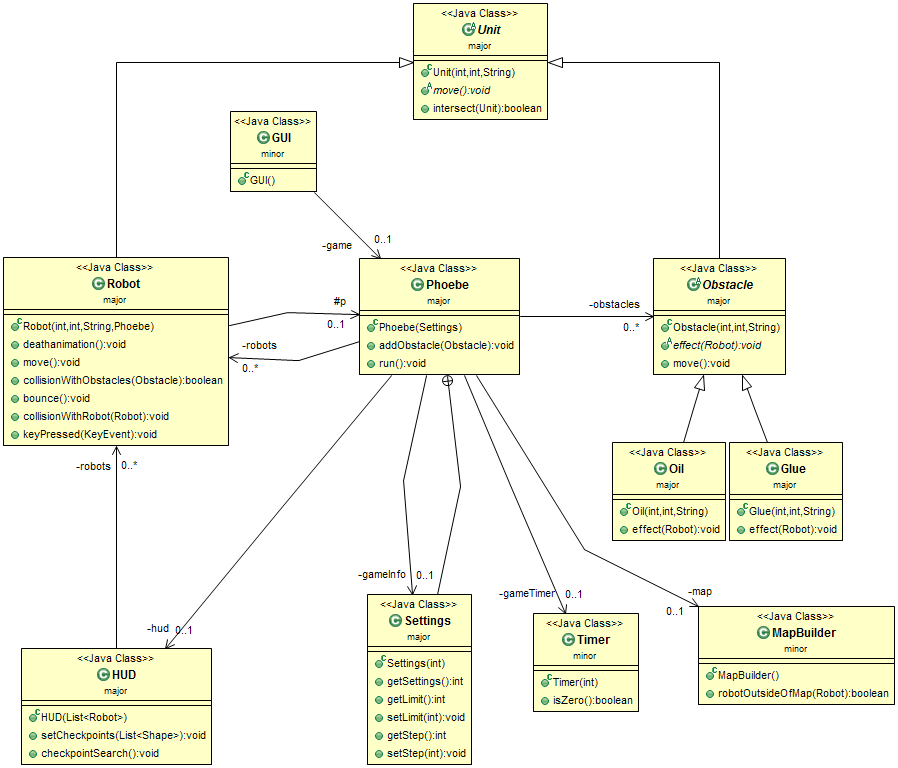
\includegraphics[width=17cm]{images/struktdiagram.PNG}
\caption{Statikus struktúra diagram}
\label{fig:example3}
\end{center}
\end{figure}
\pagebreak

\begin{figure}[h]
\begin{center}
%\includegraphics[width=17cm]{chapters/chapter04/example.pdf}
\caption{x}
\label{fig:example3}
\end{center}
\end{figure}


\section{Osztályok leírása}
\subsection{Glue}
\begin{itemize}
\item Felelősség\\
A játékban szereplő Ragacs foltok viselkedését leíró osztály
\item Ősosztályok\\
Unit$\rightarrow$Obstacle
\item Metódusok
	\begin{itemize}
	    \item \textbf{Glue}(int x, int y): Amikor létrehozunk valahol egy ragacs objektumot, akkor ez a konstruktor hívódik meg. Meghívja az ősosztály konstruktorát.
		\item void \textbf{effect}(Robot r): Ütközéskor hívja meg az ütközést vizsgáló függvénye a Robot osztálynak. Módosítja a robot slowed értékét 50\%-ra a robot slowed attribútum setterének meghívásával.
	\end{itemize}
\end{itemize}

\subsection{GUI}
\begin{itemize}
\item Felelősség\\
A grafikus felületért felelős osztály, amely a menüt és a játékot jeleníti meg.
\item Attribútumok
	\begin{itemize}
		\item \textbf{Phoebe} game: referencia a játékra
	\end{itemize}
\item Metódusok
	\begin{itemize}
		\item\textbf{GUI}(): Konstruktor. Beállítja az ablak nevét, létrehozza az ablak elemeit, elrendezi őket és beállítja a figyelőket(ActionListener).
	\end{itemize}
\end{itemize}

\subsection{HUD}
\begin{itemize}
\item Felelősség\\
A robotok ragacs- és olajkészletét, illetve megtett köreit és checkpontjait számolja. Megvalósítja a checkpoint ellenőrzést.
\item Attribútumok
	\begin{itemize}
		\item \textbf{int[]} checkpointReached: Minden robothoz külön tárolja a legutoljára érintett checkpoint sorszámát.
		\item \textbf{int[]} lap: Minden robothoz tárolja a megtett körök számát. 
		\item \textbf{int[]} numGlue: Minden robothoz tárolja a ragacsok számát.
		\item \textbf{int[]} numOil: Minden robothoz tárolja az olajok számát.
		\item \textbf{List} checkpoints: Tárolja a checkpointokat reprezentáló objektumokat List adatszerkezetben. A checkpointSearch függvény kérdezi le ebből a következő checkpoint helyzetét. 
		\item \textbf{List<Robot>} robots: A robotokat tároló List adatszerkezet. A checkpointSearch függvény kérdezi le ebből a robotokat, majd azok helyzetét.
	\end{itemize}
\item Metódusok
	\begin{itemize}
		\item \textbf{HUD}(List<Robot> robs): Konstruktor, inicializálja a köröket számláló változót, az érintett checkpointokat, a ragacs és olajkészleteket. 
		\item void \textbf{checkpointSearch}(): Ellenőrzi hogy a robotok teljesítették-e a következő checkpointot.
		\item void \textbf{setCheckpoints}(List checkObj): Checkpointokat reprezentáló adatszerkezet betöltése.
		
	\end{itemize}
\end{itemize}

\subsection{MapBuilder}
\begin{itemize}
\item Felelősség\\
A pálya felépítéséért, a checkpointok tárolásáért és a robot pályán tartózkodásának vizsgálatáért felelős osztály.
\item Attribútumok
	\begin{itemize}
		\item \textbf{List} checkpoints: Tárolja a checkpointokat reprezentáló objektumokat List adatszerkezetben.
		\item \textbf{int[]} startPosPlayerOne: Meghatároz egy (x,y) koordinátát, ahol az első játékos kezd.
		\item \textbf{int[]} startPosPlayerTwo: Meghatároz egy (x,y) koordinátát, ahol az második játékos kezd.
	\end{itemize}
\item Metódusok
	\begin{itemize}
		\item \textbf{MapBuilder}(): Konstruktor, a pálya beolvasása fájlból, majd létrehozása.
		\item boolean \textbf{robotOutsideOfMap}(Robot r): Igaz értéket ad vissza, ha a robot leesett a pályáról, hamisat ha még rajta van.
	\end{itemize}
\end{itemize}

\subsection{Obstacle}
\begin{itemize}
\item Felelősség\\
A pályán/játékosoknál lévő különböző akadályokat (ragacs,olaj) összefogó ősosztály.
\item Ősosztályok\\
Unit
\item Attribútumok
	\begin{itemize}
		\item \textbf{int} WIDTH: Az akadályokat jellemző szélesség. Szükség van rá, hogy létrehozzuk a leszármazottak hitbox-át(sokszög pályaelem).
		\item \textbf{int} HEIGHT: Az akadályokat jellemző hosszúság. Szükség van rá, hogy létrehozzuk a leszármazottak hitbox-át(sokszög pályaelem).
	\end{itemize}
\item Metódusok
	\begin{itemize}
		\item \textbf{Obstacle}(int x, int y, String imagelocation): meghívja a Unit konstruktorát a megadott adatokkal és létrehoz egy sokszög elemet ami reprezentálja a pályán majd.
		\item void \textbf{effect}(Robot r): Meghatározza, milyen hatással van a robotra, ha érintkezik egy Obstacle-lel. Absztrakt.
	\end{itemize}
\end{itemize}

\subsection{Oil}
\begin{itemize}
\item Felelősség\\
A pályára lerakható olaj megvalósítása. Ha belelép egy játékos egy ilyen olajfoltba, az effect függvény letiltja a mozgatást az adott roboton a következő ugrásig.
\item Ősosztályok\\
Unit $\rightarrow$ Obstacle 
\item Metódusok
	\begin{itemize}
		\item \textbf{Oil}(int x, int y, String imagelocation): Egy Oil elem létrehozásáért felelős.
		\item void \textbf{effect}(Robot r): Meghatározza, milyen hatással van a robotra, ha beleugrik egy olajfoltba. Ebben az esetben letiltja a játékost, hogy irányt váltson.
	\end{itemize}
\end{itemize}

\subsection{Phoebe}
\begin{itemize}
\item Felelősség\\
A játék motorját képviselő osztály. A robotok pozíciójáért, az akadályok elhelyezéséért és a játék végéért felel.
\item Attribútumok
	\begin{itemize}
		\item \textbf{boolean} ended: Állapot változó, ha vége a játéknak, akkor true. Ha beteljesül egy játék végét jelentő esemény, akkor ezen a változón keresztül leáll a játék és megállapítódik a nyertes.
		\item \textbf{List<Robot>} robots: A játékban szereplő robotok listája.
		\item \textbf{List<Obstacle>} obstacles: A játékban szereplő akadályok listája.
		\item \textbf{HUD} hud: A játékosok előrehaladását, ragacs és olajkészleteit tartja számon
		\item \textbf{MapBuilder} map: A pályát reprezentáló objektum. Tárolja még a checkpointokat és a robotok kezdő koordinátáit.
	\end{itemize}
\item Metódusok
	\begin{itemize}
		\item \textbf{Phoebe}(Setting set): A játék felépítése, a robotok lista, az akadályok lista létrehozása
		\item void \textbf{run}(): Ez a metódus futtatja a főciklust, amelyben maga a játék működik.
	\end{itemize}
\end{itemize}

\subsection{Robot}
\begin{itemize}
\item Felelősség\\
A játékban résztvevő robotok viselkedését és kezelését leíró osztály.
\item Ősosztályok\\
Unit
\item Interfészek\\
Nincs interfésze
\item Attribútumok
	\begin{itemize}
		\item \textbf{int} staticID: Az osztályhoz tartozó statikus azonosító, a példány                azonosítójának(id) meghatározásához szükséges.
		\item \textbf{int} HEIGHT: A robot képének magassága, collision                      detektálásnál, továbbá az irányítást segítő nyíl kezdő koordinátájának                  meghatározásánál szükséges.
		\item \textbf{int} WIDTH: A robot képének szélessége, funkcionalitásban hasonló a WIDTH-hez.
		\item \textbf{int} ID: A robot példányának egyedi azonosítója, a keyconfig sorának                     indexelésére szükséges.
		\item \textbf{double} slowed: A sebesség módosításáért felel, default értéke 1.0. Amennyiben ragacsba lép a robot ez 0.5-re módosul és minden ugrás végén visszaáll az eredeti értékére. Ugrásnál ezzel szorozzuk be a végkordinátát kiszámító sugár hosszát.
		\item \textbf{boolean} oiled: Azt jelzi, hogy olajba lépett-e. Ennek hatására a mozgás iránya módosíthatatlanná válik egy kis időre. 
		\item \textbf{int} arrowendx: A robot irányítását segítő nyílnak az x koordinátája, a nyíl kirajzolásánál van szerepe.
		\item \textbf{int} arrowendy: A robot irányítását segítő nyílnak az y koordinátája, a nyíl kirajzolásánál van szerepe.
		\item \textbf{double} alpha: A robot irányítását segítő nyíl vízszintessel bezárt szöge. A nyil kirajzolásánál, az ugrás végpontjának meghatározánál van szerepe.
		\item \textbf{boolean} moved: Azt jelöli, hogy lépett-e már a robot az aktuális körben. A megjelenítésnél (a nyilat ugrás közben nem jelenítjük meg), illetve az irányítás letiltásánál van szerepe (olajba lépés esetén).
\end{itemize}
\item Metódusok\\
	\begin{itemize}
		\item \textbf{Robot}(int x,int y,String imagelocation,Phoebe p): Létrehoz egy robotot a megadott x,y koordinátákon, betölti a képét az imagelocation cím alapján, továbbá eltárolja a játékmotor referenciáját.
		\item \textbf{void deathanimation}(): A Robot halálának grafikus megjelenítéséért felelős függvény.
		\item boolean \textbf{collisionWithObstacle}(Obstacle o): Ellenőrzi hogy a robot ütközött-e az akadállyal. Igazzal tér vissza ha igen, hamissal ha nem.
		\item void \textbf{collisionWithRobot}(Robot r): Ellenőrzi, hogy a robot ütközött-e másik robottal. Ha igen, akkor gondoskodik róla, hogy a robotok a megfelelő szögben pattanjanak le egymásról.
		\item void \textbf{keyPressed}(): A robot irányítását megvalósító függvény, a játékmotor keylistener-e által hívódik meg, a lenyomott billentyű keyevent-jére. A következő ugrás beállítása, a ragacs/olaj lerakása történhet itt a keyconfig változó felhasználásával.
	\end{itemize}
\end{itemize}

\subsection{Timer}
\begin{itemize}
\item Felelősség\\
A visszaszámlálásért (idő, director time) felelős.
\item Metódusok
	\begin{itemize}
		\item \textbf{Timer}(int i): Konstruktor; inicializál egy viszaszámláló órát.
		\item boolean \textbf{isZero}(): Igazzal tér vissza, ha a megadott idő lejárt.
	\end{itemize}
\end{itemize}

\subsection{Unit}
\begin{itemize}
\item Felelősség\\
A pályán található objektumokért felel és azok viszonyáról (például ütközésükről).
\item Attribútumok
	\begin{itemize}
		\item \textbf{int} x: Az egység x koordinátája
		\item \textbf{int} y: Az egység y koordinátája
		\item \textbf{Object} hitbox: Az egységet a pályán reprezentáló sokszög.
	\end{itemize}
\item Metódusok
	\begin{itemize}
		\item void \textbf{move}() : Absztrakt függvény, mely a leszármazottakban fog megvalósulni. Az egységek mozgásáért felelős.
		\item boolean \textbf{intersect}(Unit u): Két egység ütközését meghatározó függvény.
	\end{itemize}
\end{itemize}
\pagebreak

\section{Szekvencia diagramok}

\subsection{Robot::CheckpointSearch}
\begin{figure}[h]
\begin{center}
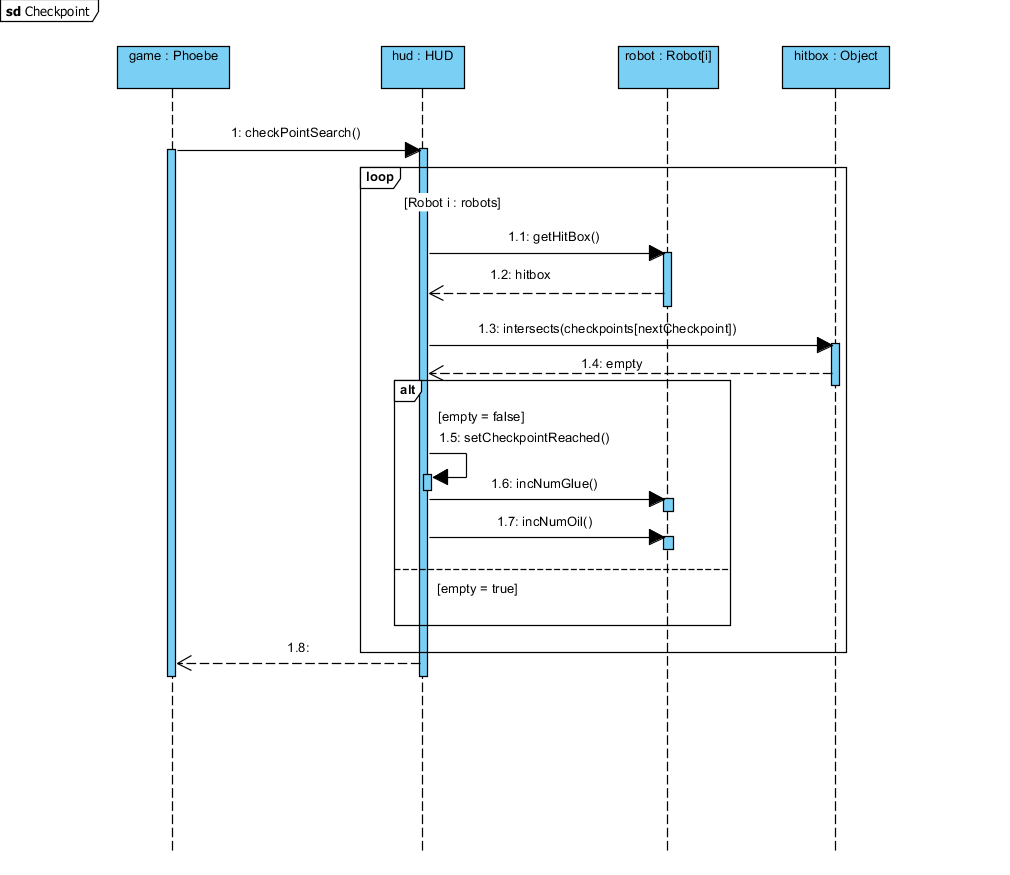
\includegraphics[width=17cm]{images/CheckpointSearch.PNG}
\caption{Következő checkpoint vizsgálata}
\label{fig:example2}
\end{center}
\end{figure}
\pagebreak

\subsection{Robot::CollisonWithObstacle}
\begin{figure}[h]
\begin{center}
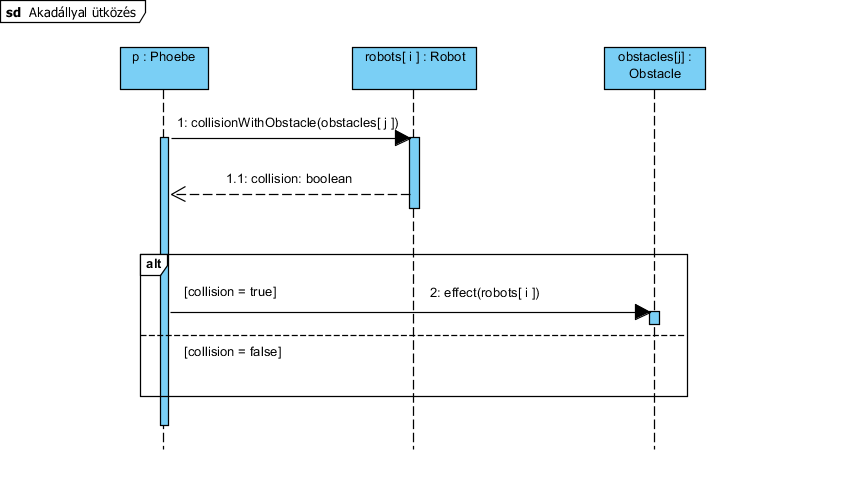
\includegraphics[width=17cm]{images/collisionWithObstacle()_sequence.PNG}
\caption{Robot ütközése akadállyal}
\label{fig:example4}
\end{center}
\end{figure}
\pagebreak

\subsection{Robot::CollisionWithRobot}
\begin{figure}[h]
\begin{center}
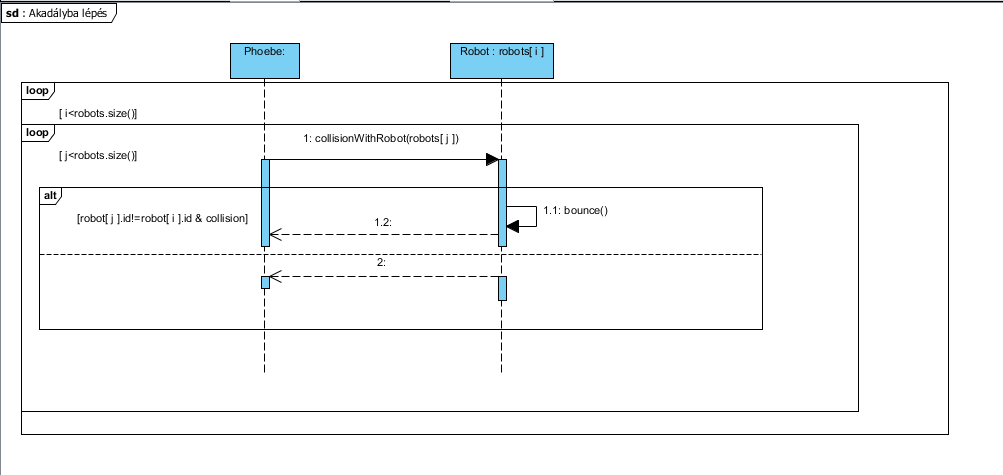
\includegraphics[width=17cm]{images/collisionWithRobot()_sequence.PNG}
\caption{Robot ütközése másik robottal}
\label{fig:example5}
\end{center}
\end{figure}
\pagebreak

\subsection{Robot::FallDown}
\begin{figure}[h]
\begin{center}
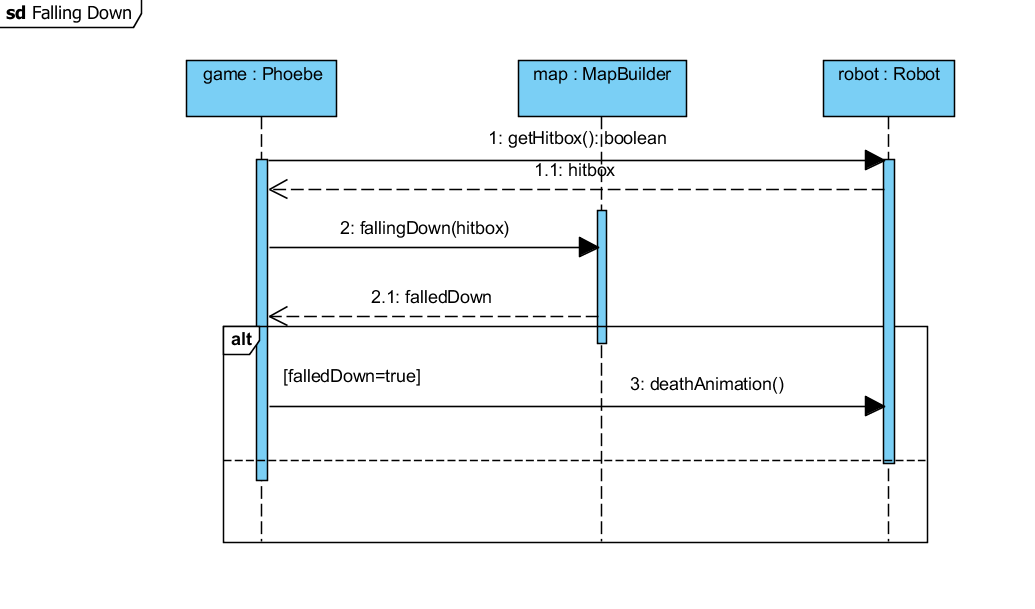
\includegraphics[width=17cm]{images/FallingDown.PNG}
\caption{Robot leesése a pályáról}
\label{fig:example6}
\end{center}
\end{figure}
\pagebreak

\subsection{Robot::InitGame}
\begin{figure}[h]
\begin{center}
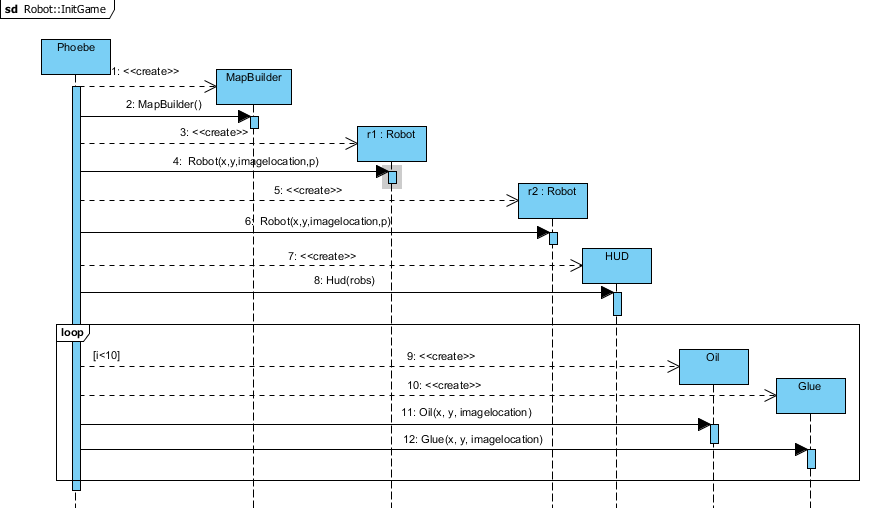
\includegraphics[width=17cm]{images/RobotInitGame.PNG}
\caption{A játék inicializálása}
\label{fig:example7}
\end{center}
\end{figure}
\pagebreak

\subsection{Robot::Move}
\begin{figure}[h]
\begin{center}
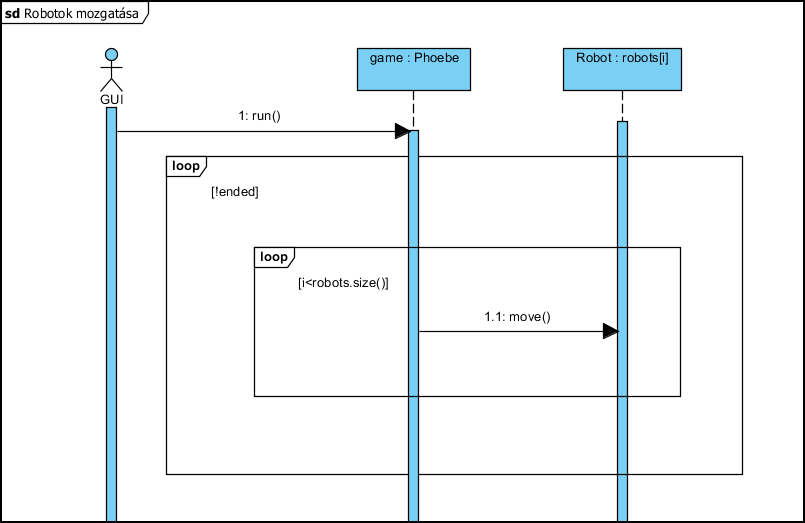
\includegraphics[width=17cm]{images/RobotMove.png}
\caption{A robot mozgatása}
\label{fig:example8}
\end{center}
\end{figure}
\pagebreak

\subsection{Robot::NewObstacle}
\begin{figure}[h]
\begin{center}
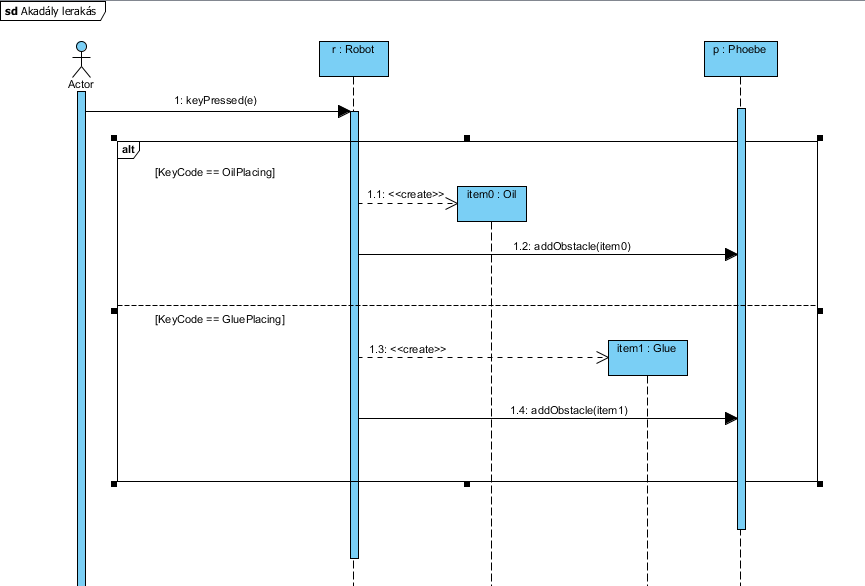
\includegraphics[width=17cm]{images/RobotAddObstacle.png}
\caption{Akadály lerakása}
\label{fig:example9}
\end{center}
\end{figure}
\pagebreak

\subsection{Robot::Settings}
\begin{figure}[h]
\begin{center}
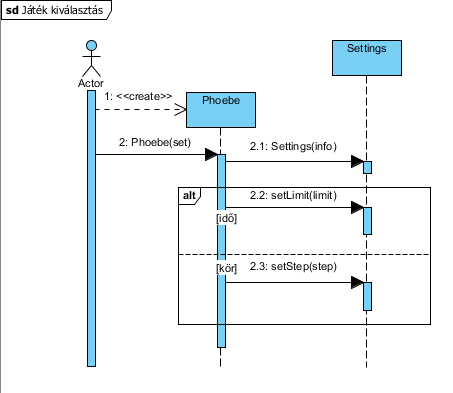
\includegraphics[width=17cm]{images/kivalasztas.PNG}
\caption{A játék beállításainak kiválasztása}
\label{fig:example10}
\end{center}
\end{figure}
\pagebreak

\subsection{Robot::End}
\begin{figure}[h]
\begin{center}
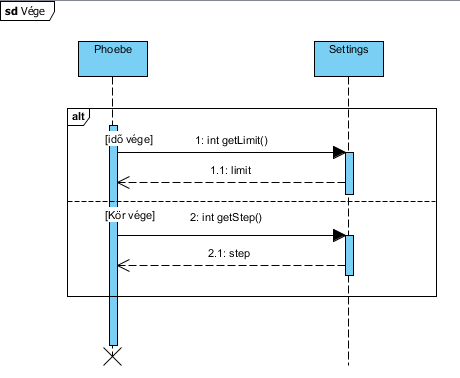
\includegraphics[width=17cm]{images/end.PNG}
\caption{Játék vége}
\label{fig:example11}
\end{center}
\end{figure}
\pagebreak

\section{State-chartok}

\subsection{Robot::States}
\begin{figure}[h]
\begin{center}
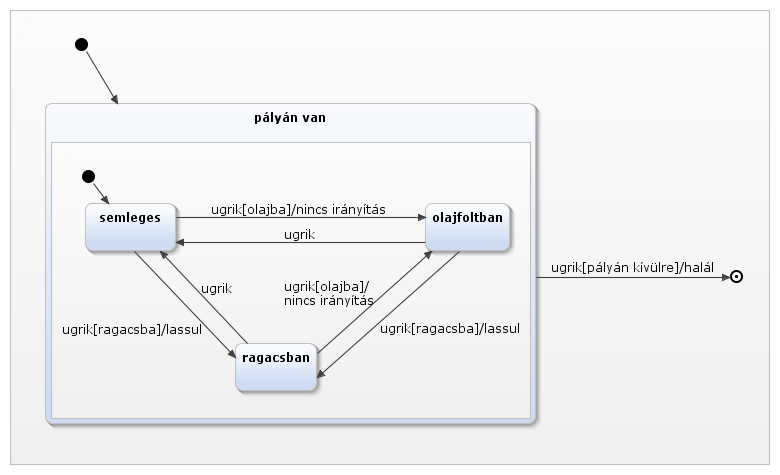
\includegraphics[width=17cm]{images/robot.png}
\caption{A robot állapotai}
\label{fig:example12}
\end{center}
\end{figure}